
\documentclass[a4paper,11pt]{article}
\usepackage{graphicx}

\begin{document}

\title{CS251 Box2D Project}
\author{Group 20}
\maketitle
The original idea of the project was to make a set of obstracles for a car and we succeeded in getting most of it but there was problem with the creation of the horizontal escaltor. \\ 
So we made a different obstracle instead of the horizontal escalator. \\ 
And also we added the rottatng platform at the top instead of a static platform. \\
\begin{figure}[h]
\centering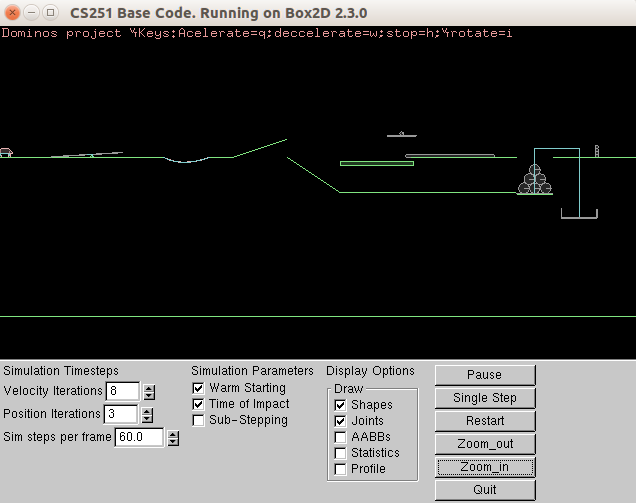
\includegraphics[width=0.4\linewidth]{doc/example}
\caption{A screenshot of the project}
\end{figure}
\section{Observations:}
The top 5 functions in this version are
\begin{itemize}
 \item operator-(b2Vec2 const\&, b2Vec2 const\&)
 \item b2Dot(b2Vec2 const\&, b2Vec2 const\&)
 \item b2Vec2::b2Vec2(float, float)
 \item operator\*(float, b2Vec2 const\&)
 \item operator+(b2Vec2 const\&, b2Vec2 const\&)
\end{itemize}
\begin{figure}[h]
\centering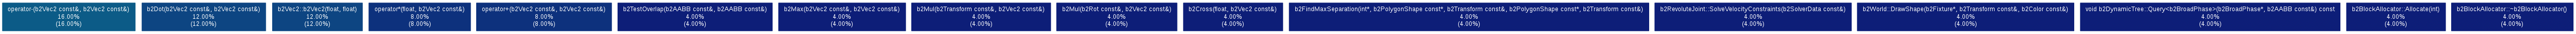
\includegraphics[width=0.4\linewidth]{doc/profile}
\caption{A call graph}
\end{figure}
We included a button so that even the car will be able to rotate, so that even when the car gets inverted it gets back onto its wheels by rotating 
\section{Difficulties:}
\begin{itemize}
\item Addition of buttons and introducing mouse click was a problem. Read the callbacks.cpp and hpp files to get to know how to add the buttons.
\item Understanding static function and their use for introducing button and also discovering the callbacks in main.cpp
\item Didn't know that we need to make changes in main.cpp also. Debugged it by running each file.
\item Making string was also challenge.
\end{itemize}
\end{document}
